\chapter{Dyskusja rezultatów}

\section{Przykładowe wyniki}
Wracając do dziennika zdarzeń, który był w sekcji i dla którego przykładowych modeli obliczono w sekcji model dla tego logu znaleziony przy pomocy tego algorytmu to 
\begin{figure}[!ht]
	\centering{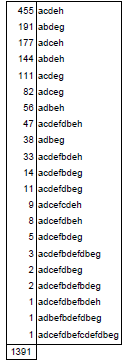
\includegraphics[scale=0.5]{example-event-log.png}}
	\caption{\label{fig:flow_chart}Dziennik zdarzeń}
\end{figure}

Inne przykłady działania to: 

\section{Wyniki w zależności od przyjętych wag poszczególnych metryk}

\subsection{Złożoność}

\section{Wnioski}
